% !TeX root = thesis.tex
%--------------------------------------------------------------------%
%
% Template TA LaTeX Teknik Informatika ITERA.
% Editor: Radhinka Bagaskara, Martin C.T. Manullang, iwawiwi
% Version 2022-0.1
%
% Berdasarkan "Templat LaTeX Tesis Informatika ITB" oleh Petra Barus & Peb Ruswono Aryan
% https://github.com/petrabarus/if-itb-latex
%--------------------------------------------------------------------%
%
% Berkas ini berisi struktur utama dokumen LaTeX yang akan dibuat.
%
%--------------------------------------------------------------------%

\documentclass[12pt, a4paper, onecolumn, oneside, final]{report}

%-------------------------------------------------------------------%
%
% Konfigurasi dokumen LaTeX untuk laporan tesis IF ITB
%
% @author Petra Novandi
%
%-------------------------------------------------------------------%
%
% Berkas asli berasal dari Steven Lolong
%
%-------------------------------------------------------------------%

% Ukuran kertas
\special{papersize=210mm,297mm}

% Setting margin
\usepackage[top=3cm,bottom=3cm,left=4cm,right=3cm]{geometry}

\usepackage{mathptmx}

% Judul bahasa Indonesia
\usepackage[bahasa]{babel}

% Format citation
\usepackage[backend=bibtex,citestyle=ieee]{biblatex}

\usepackage[utf8]{inputenc}
\usepackage{graphicx}
\usepackage{titling}
\usepackage{blindtext}
\usepackage{sectsty}
\usepackage{chngcntr}
\usepackage{etoolbox}
\usepackage[bookmarks]{hyperref}
\hypersetup{
    colorlinks,
    citecolor=black,
    filecolor=black,
    linkcolor=black,
    urlcolor=black
}% Package untuk link di daftar isi.
\usepackage{titlesec}       % Package Format judul
\usepackage{parskip}
\usepackage{ragged2e}		% Alignment
\usepackage{multirow}		% Untuk bisa merge cell di tabel
\usepackage{tikz}			% Untuk menggambar kotak pas foto
\usepackage{setspace}		% Spacing paragraph
\usepackage{fancyhdr}		% Agar nomor halaman di pojok kanan atas
\usepackage{caption} 		% Caption gambar & tabel

% Setting supaya nomor halaman pertama dengan "chapter"
% berada di kanan atas
\fancypagestyle{plain}{%
	\fancyhf{}%
	\renewcommand{\headrulewidth}{0pt}
	\fancyhead[R]{\thepage}
}

% Line satu setengah spasi
\renewcommand{\baselinestretch}{1.5}

% Setting judul
\chapterfont{\centering \large}
\titleformat{\chapter}[display]%
  	{\large\centering\bfseries}%
  	{\chaptertitlename\ \thechapter}{0pt}%
  	{\large\bfseries\uppercase}
\titleformat{\section}%
	{\normalfont\normalsize\bfseries}{\thesection}{1em}{}
\titleformat{\subsection}%
	{\normalfont\normalsize\bfseries}{\thesubsection}{1em}{}
    
% Setting spacing di setiap judul chapter
\titlespacing*{\chapter}{0pt}{-30pt}{20pt}

% Setting nomor pada subbsubsubbab
\setcounter{secnumdepth}{3}

\makeatletter
% Command untuk variabel NIM
\newcommand{\nim}[1]{\def\@nim{#1}}
\newcommand{\printnim}{\@nim}

% Command untuk variabel Dosen Pembimbing I & II
\newcommand{\namadosbinga}[1]{\def\@namadosbinga{#1}}
\newcommand{\namadosbingb}[1]{\def\@namadosbingb{#1}}
\newcommand{\nipdosbinga}[1]{\def\@nipdosbinga{#1}}
\newcommand{\nipdosbingb}[1]{\def\@nipdosbingb{#1}}
\newcommand{\printnamadosbinga}{\@namadosbinga}
\newcommand{\printnamadosbingb}{\@namadosbingb}
\newcommand{\printnipdosbinga}{\@nipdosbinga}
\newcommand{\printnipdosbingb}{\@nipdosbingb}
\newcommand{\dosbingA}[2]{\namadosbinga{#1} \nipdosbinga{#2}}
\newcommand{\dosbingB}[2]{\namadosbingb{#1} \nipdosbingb{#2}}

\makeatother

% Counter untuk figure dan table.
\counterwithin{figure}{section}
\counterwithin{table}{section}

% Supaya tidak ada garis di header
\renewcommand{\headrulewidth}{0pt}

% Setting penomoran caption gambar
\renewcommand{\thefigure}{\arabic{chapter}.\arabic{figure}}

% Setting penomoran caption tabel
\renewcommand{\thetable}{\arabic{chapter}.\arabic{figure}}

% Mengkapitalkan judul Daftar Isi, Gambar, & Tabel
\addto\captionsbahasa{%
	\renewcommand{\contentsname}{DAFTAR ISI}%
	\renewcommand{\listfigurename}{DAFTAR GAMBAR}%
	\renewcommand{\listtablename}{DAFTAR TABEL}%
}

% english title
\providecommand\titleEN[1]{\providecommand\thetitleEN{#1}}

% Saya lupa ini buat apa (Radhinka)
%\renewcommand{\theHsection}{\thepart.section.\thesection}



\makeatletter

\makeatother

\bibliography{references}

\begin{document}
    \sloppy % mencegah text overflow.
    \chapter{Tinjauan Pustaka}

Bab Studi Literatur digunakan untuk mendeskripsikan kajian literatur yang terkait dengan persoalan tugas akhir. Tujuan studi literatur adalah:

\begin{enumerate}
    \item menunjukkan kepada pembaca adanya gap seperti pada rumusan masalah yang memang belum terselesaikan,
    \item memberikan pemahaman yang secukupnya kepada pembaca tentang teori atau pekerjaan terkait yang terkait langsung dengan penyelesaian persoalan, serta
    \item menyampaikan informasi apa saja yang sudah ditulis/dilaporkan oleh pihak lain (peneliti/Tugas Akhir/Tesis) tentang hasil penelitian/pekerjaan mereka yang sama atau mirip kaitannya dengan persoalan tugas akhir.
\end{enumerate}

\blindtext

\section{Dasar Teori}
Perujukan literatur dapat dilakukan dengan menambahkan entri baru di berkas. Tulisan ini merujuk pada \cite{knuth2001art}

    \subsection{Subbab}

    \blindtext

    \begin{figure}[h]
        \centering
        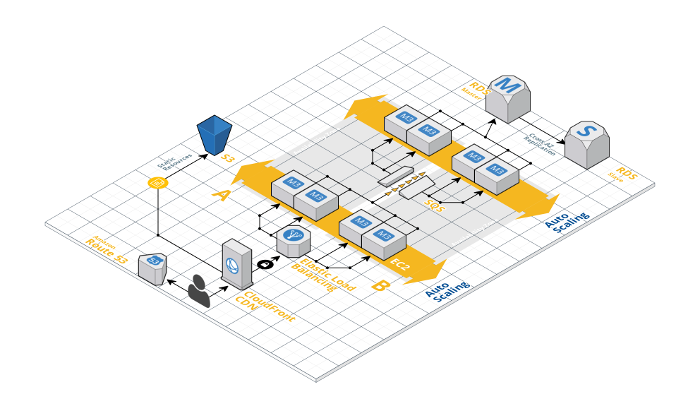
\includegraphics[width=0.8\textwidth]{figures/chapter-2-infrastructure-diagram.png}
        \caption{Contoh gambar}
        \label{fig:1}
    \end{figure}

    \subsubsection{Subsubbab}

    \blindtext
	
	\begin{table}[h!]
		\centering
		\caption{Contoh tabel}
		\begin{tabular}{|c|c|c|c|} 
			\hline
			Col1 & Col2 & Col2 & Col3 \\
			\hline
			1 & 6 & 87837 & 787 \\ 
			\hline
			2 & 7 & 78 & 5415 \\
			\hline
			3 & 545 & 778 & 7507 \\
			\hline
			4 & 545 & 18744 & 7560 \\
			\hline
			5 & 88 & 788 & 6344 \\
			\hline
		\end{tabular}
		\label{table:1}
	\end{table}
	
\section{Studi Terkait}
\blindtext


    %----------------------------------------------------------------%
    % Konfigurasi Bab
    %----------------------------------------------------------------%
    \renewcommand{\chaptername}{BAB}
    % Bab: Arabic
    \renewcommand{\thechapter}{\Roman{chapter}}
    % Sub-bab: Roman
    \renewcommand\thesection{\arabic{chapter}.\arabic{section}}
    
    % Setting supaya nomor halaman pertama dengan "chapter"
    % berada di tengah bawah
    \fancypagestyle{plain}{%
    	\fancyhf{}%
    	\renewcommand{\headrulewidth}{0pt}
    	\fancyhead[]{}
    	\fancyfoot[C]{\thepage}
    }
    %----------------------------------------------------------------%

    %----------------------------------------------------------------%
    % Daftar Bab
    % Untuk menambahkan daftar bab, buat berkas bab misalnya `chapter-6` di direktori `chapters`, dan masukkan ke sini.
    %----------------------------------------------------------------%

    % Reset penomoran halaman menjadi 1
    \clearpage
    \setcounter{page}{1}
    \pagenumbering{arabic}

    \justifying
    \chapter{Tinjauan Pustaka}

Bab Studi Literatur digunakan untuk mendeskripsikan kajian literatur yang terkait dengan persoalan tugas akhir. Tujuan studi literatur adalah:

\begin{enumerate}
    \item menunjukkan kepada pembaca adanya gap seperti pada rumusan masalah yang memang belum terselesaikan,
    \item memberikan pemahaman yang secukupnya kepada pembaca tentang teori atau pekerjaan terkait yang terkait langsung dengan penyelesaian persoalan, serta
    \item menyampaikan informasi apa saja yang sudah ditulis/dilaporkan oleh pihak lain (peneliti/Tugas Akhir/Tesis) tentang hasil penelitian/pekerjaan mereka yang sama atau mirip kaitannya dengan persoalan tugas akhir.
\end{enumerate}

\blindtext

\section{Dasar Teori}
Perujukan literatur dapat dilakukan dengan menambahkan entri baru di berkas. Tulisan ini merujuk pada \cite{knuth2001art}

    \subsection{Subbab}

    \blindtext

    \begin{figure}[h]
        \centering
        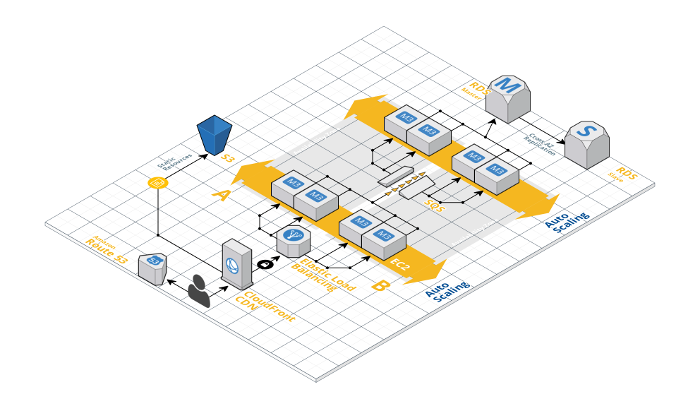
\includegraphics[width=0.8\textwidth]{figures/chapter-2-infrastructure-diagram.png}
        \caption{Contoh gambar}
        \label{fig:1}
    \end{figure}

    \subsubsection{Subsubbab}

    \blindtext
	
	\begin{table}[h!]
		\centering
		\caption{Contoh tabel}
		\begin{tabular}{|c|c|c|c|} 
			\hline
			Col1 & Col2 & Col2 & Col3 \\
			\hline
			1 & 6 & 87837 & 787 \\ 
			\hline
			2 & 7 & 78 & 5415 \\
			\hline
			3 & 545 & 778 & 7507 \\
			\hline
			4 & 545 & 18744 & 7560 \\
			\hline
			5 & 88 & 788 & 6344 \\
			\hline
		\end{tabular}
		\label{table:1}
	\end{table}
	
\section{Studi Terkait}
\blindtext

    \chapter{Tinjauan Pustaka}

Bab Studi Literatur digunakan untuk mendeskripsikan kajian literatur yang terkait dengan persoalan tugas akhir. Tujuan studi literatur adalah:

\begin{enumerate}
    \item menunjukkan kepada pembaca adanya gap seperti pada rumusan masalah yang memang belum terselesaikan,
    \item memberikan pemahaman yang secukupnya kepada pembaca tentang teori atau pekerjaan terkait yang terkait langsung dengan penyelesaian persoalan, serta
    \item menyampaikan informasi apa saja yang sudah ditulis/dilaporkan oleh pihak lain (peneliti/Tugas Akhir/Tesis) tentang hasil penelitian/pekerjaan mereka yang sama atau mirip kaitannya dengan persoalan tugas akhir.
\end{enumerate}

\blindtext

\section{Dasar Teori}
Perujukan literatur dapat dilakukan dengan menambahkan entri baru di berkas. Tulisan ini merujuk pada \cite{knuth2001art}

    \subsection{Subbab}

    \blindtext

    \begin{figure}[h]
        \centering
        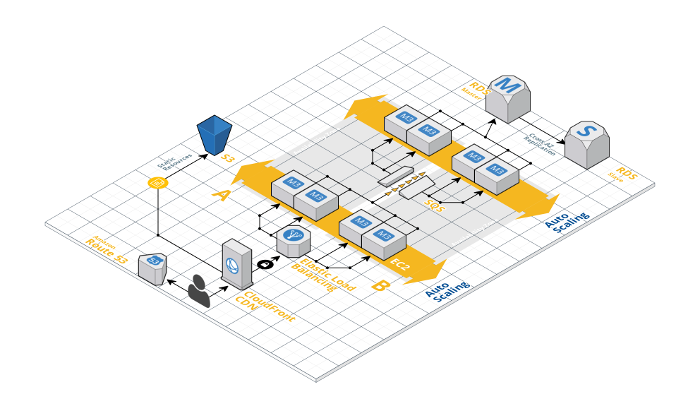
\includegraphics[width=0.8\textwidth]{figures/chapter-2-infrastructure-diagram.png}
        \caption{Contoh gambar}
        \label{fig:1}
    \end{figure}

    \subsubsection{Subsubbab}

    \blindtext
	
	\begin{table}[h!]
		\centering
		\caption{Contoh tabel}
		\begin{tabular}{|c|c|c|c|} 
			\hline
			Col1 & Col2 & Col2 & Col3 \\
			\hline
			1 & 6 & 87837 & 787 \\ 
			\hline
			2 & 7 & 78 & 5415 \\
			\hline
			3 & 545 & 778 & 7507 \\
			\hline
			4 & 545 & 18744 & 7560 \\
			\hline
			5 & 88 & 788 & 6344 \\
			\hline
		\end{tabular}
		\label{table:1}
	\end{table}
	
\section{Studi Terkait}
\blindtext

    \chapter{Tinjauan Pustaka}

Bab Studi Literatur digunakan untuk mendeskripsikan kajian literatur yang terkait dengan persoalan tugas akhir. Tujuan studi literatur adalah:

\begin{enumerate}
    \item menunjukkan kepada pembaca adanya gap seperti pada rumusan masalah yang memang belum terselesaikan,
    \item memberikan pemahaman yang secukupnya kepada pembaca tentang teori atau pekerjaan terkait yang terkait langsung dengan penyelesaian persoalan, serta
    \item menyampaikan informasi apa saja yang sudah ditulis/dilaporkan oleh pihak lain (peneliti/Tugas Akhir/Tesis) tentang hasil penelitian/pekerjaan mereka yang sama atau mirip kaitannya dengan persoalan tugas akhir.
\end{enumerate}

\blindtext

\section{Dasar Teori}
Perujukan literatur dapat dilakukan dengan menambahkan entri baru di berkas. Tulisan ini merujuk pada \cite{knuth2001art}

    \subsection{Subbab}

    \blindtext

    \begin{figure}[h]
        \centering
        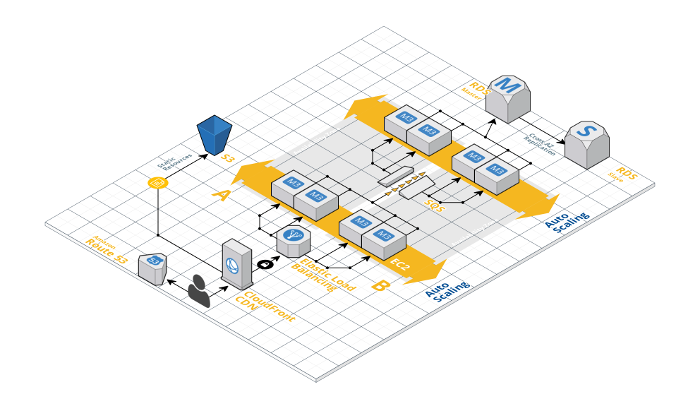
\includegraphics[width=0.8\textwidth]{figures/chapter-2-infrastructure-diagram.png}
        \caption{Contoh gambar}
        \label{fig:1}
    \end{figure}

    \subsubsection{Subsubbab}

    \blindtext
	
	\begin{table}[h!]
		\centering
		\caption{Contoh tabel}
		\begin{tabular}{|c|c|c|c|} 
			\hline
			Col1 & Col2 & Col2 & Col3 \\
			\hline
			1 & 6 & 87837 & 787 \\ 
			\hline
			2 & 7 & 78 & 5415 \\
			\hline
			3 & 545 & 778 & 7507 \\
			\hline
			4 & 545 & 18744 & 7560 \\
			\hline
			5 & 88 & 788 & 6344 \\
			\hline
		\end{tabular}
		\label{table:1}
	\end{table}
	
\section{Studi Terkait}
\blindtext

    \chapter{Tinjauan Pustaka}

Bab Studi Literatur digunakan untuk mendeskripsikan kajian literatur yang terkait dengan persoalan tugas akhir. Tujuan studi literatur adalah:

\begin{enumerate}
    \item menunjukkan kepada pembaca adanya gap seperti pada rumusan masalah yang memang belum terselesaikan,
    \item memberikan pemahaman yang secukupnya kepada pembaca tentang teori atau pekerjaan terkait yang terkait langsung dengan penyelesaian persoalan, serta
    \item menyampaikan informasi apa saja yang sudah ditulis/dilaporkan oleh pihak lain (peneliti/Tugas Akhir/Tesis) tentang hasil penelitian/pekerjaan mereka yang sama atau mirip kaitannya dengan persoalan tugas akhir.
\end{enumerate}

\blindtext

\section{Dasar Teori}
Perujukan literatur dapat dilakukan dengan menambahkan entri baru di berkas. Tulisan ini merujuk pada \cite{knuth2001art}

    \subsection{Subbab}

    \blindtext

    \begin{figure}[h]
        \centering
        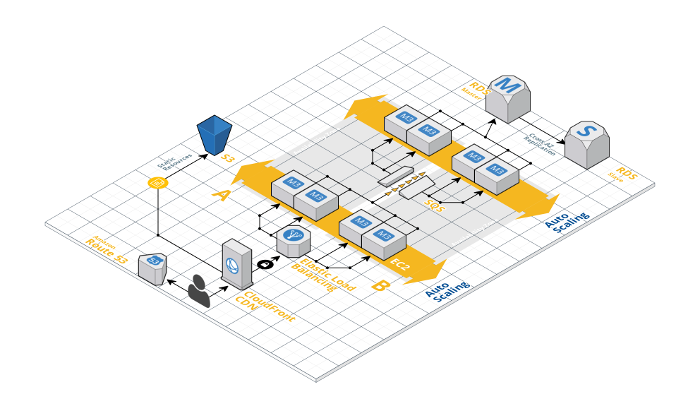
\includegraphics[width=0.8\textwidth]{figures/chapter-2-infrastructure-diagram.png}
        \caption{Contoh gambar}
        \label{fig:1}
    \end{figure}

    \subsubsection{Subsubbab}

    \blindtext
	
	\begin{table}[h!]
		\centering
		\caption{Contoh tabel}
		\begin{tabular}{|c|c|c|c|} 
			\hline
			Col1 & Col2 & Col2 & Col3 \\
			\hline
			1 & 6 & 87837 & 787 \\ 
			\hline
			2 & 7 & 78 & 5415 \\
			\hline
			3 & 545 & 778 & 7507 \\
			\hline
			4 & 545 & 18744 & 7560 \\
			\hline
			5 & 88 & 788 & 6344 \\
			\hline
		\end{tabular}
		\label{table:1}
	\end{table}
	
\section{Studi Terkait}
\blindtext

    \chapter{Tinjauan Pustaka}

Bab Studi Literatur digunakan untuk mendeskripsikan kajian literatur yang terkait dengan persoalan tugas akhir. Tujuan studi literatur adalah:

\begin{enumerate}
    \item menunjukkan kepada pembaca adanya gap seperti pada rumusan masalah yang memang belum terselesaikan,
    \item memberikan pemahaman yang secukupnya kepada pembaca tentang teori atau pekerjaan terkait yang terkait langsung dengan penyelesaian persoalan, serta
    \item menyampaikan informasi apa saja yang sudah ditulis/dilaporkan oleh pihak lain (peneliti/Tugas Akhir/Tesis) tentang hasil penelitian/pekerjaan mereka yang sama atau mirip kaitannya dengan persoalan tugas akhir.
\end{enumerate}

\blindtext

\section{Dasar Teori}
Perujukan literatur dapat dilakukan dengan menambahkan entri baru di berkas. Tulisan ini merujuk pada \cite{knuth2001art}

    \subsection{Subbab}

    \blindtext

    \begin{figure}[h]
        \centering
        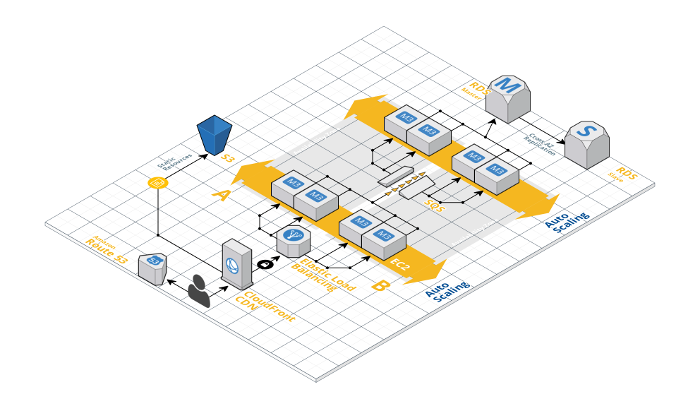
\includegraphics[width=0.8\textwidth]{figures/chapter-2-infrastructure-diagram.png}
        \caption{Contoh gambar}
        \label{fig:1}
    \end{figure}

    \subsubsection{Subsubbab}

    \blindtext
	
	\begin{table}[h!]
		\centering
		\caption{Contoh tabel}
		\begin{tabular}{|c|c|c|c|} 
			\hline
			Col1 & Col2 & Col2 & Col3 \\
			\hline
			1 & 6 & 87837 & 787 \\ 
			\hline
			2 & 7 & 78 & 5415 \\
			\hline
			3 & 545 & 778 & 7507 \\
			\hline
			4 & 545 & 18744 & 7560 \\
			\hline
			5 & 88 & 788 & 6344 \\
			\hline
		\end{tabular}
		\label{table:1}
	\end{table}
	
\section{Studi Terkait}
\blindtext

    %----------------------------------------------------------------%

    % Daftar pustaka
    \renewcommand{\bibname}{Daftar Pustaka}
    \phantomsection% 
    \addcontentsline{toc}{chapter}{Daftar Pustaka}
    \printbibliography
    

    % Index
    \appendix

    \addcontentsline{toc}{part}{Lampiran}
    \part*{Lampiran}

    \chapter{Instrumen Pengujian}
    \chapter{Rincian Kasus Uji}

\end{document}
